\section{Failure Detection and Mitigation}\label{sec:design-mig}

When network errors occur during active communication, CCLs typically trigger crashes that disrupt the entire ML job. R2CC intercepts these errors before they escalate into fatal crashes. In this section, we discuss R2CC's real-time failure detection and mitigation mechanism that consists of
(1) \textit{bilateral failure awareness} to quickly determine that a problem exists, (2) \textit{precise fault localization} to identify where the failure is, and (3) \textit{live migration} to continue the communication with alternative connections. We also introduce \textit{degradation signaling and restore} to detect recovered paths and restore the original route.

\subsection{Bilateral Error Awareness}

When a network error occurs, the server node that detects the fault typically crashes, while others in the collective remain unaware and continue polling for progress that will never occur. This asymmetric failure visibility stems from collective frameworks like NCCL, whose asynchronous, pipelined backends (e.g., RDMA, TCP) provide no fine-grained, in-band failure signaling. RDMA in this case is especially problematic: NICs autonomously handle retries and one-sided operations, delaying error propagation to the CPU.

\smallskip\textbf{Our approach:} R2CC provides bilateral failure awareness through an out-of-band (OOB) notification path. When either endpoint detects an error, it immediately alerts its peer via a separate bootstrap network, using MPI over a non-datapath NIC. This prevents peers from spinning for a long time on dead connections, reducing detection time from minutes to milliseconds.

\subsection{Precise Fault Localization}
A connection failure may stem from either endpoint, such as faulty NIC hardware, driver issues, or the physical link, but RDMA exposes only coarse transport errors (e.g., retry-exceeded), which lack the granularity to identify the impaired side. Localization therefore focuses on determining whether the failure is \textit{local}, \textit{remote}, or \textit{bilateral} to guide subsequent schedule optimization. 

\textbf{Our approach:}
R2CC introduces dedicated probe QP pools, isolated from data paths, to localize failures. When an error is detected, R2CC performs \textit{three-point triangulation} (for communicators spanning $\ge$3 servers): both endpoints and an auxiliary NIC on a third server of the same communicator issue zero-byte RDMA Writes as probes. A failed NIC produces immediate local probe errors, while its peer observes timeouts; a broken link yields timeouts at both endpoints, with the auxiliary NIC distinguishing single-endpoint vs. dual-endpoint impairment. By correlating probe outcomes, R2CC precisely identifies the fault and broadcasts it to all ranks via the OOB channel. For communicators spanning only two servers, R2CC directly marks both endpoints of the failed path unavailable and resumes on the backup connection. R2CC also periodically reprobes to detect component recovery (e.g., NIC resets, cable fixes), adapting probe frequency and strategy based on observed failure and recovery patterns.

\subsection{Live Migration for Failure Mitigation}
After detecting and localizing a failure, the system must quickly resume collectives using the remaining healthy links (Figure~\ref{fig:new-hotrepair}). This requires fast, lossless connection migration so in-flight data is preserved with two challenges: (1) backup NICs cannot access GPU buffers unless those buffers were pre-registered with them, and (2) both sender and receiver must maintain data integrity during migration.

\paragraph{Technique I: Eager provisioning of the failover fast path.} R2CC eagerly provisions the failover fast path at communicator creation. This provisioning has two scopes: \emph{GPU buffer multi-registration} is a local memory-mapping decision, whereas \emph{backup QP pre-establishment} is a neighbor-edge decision.

\textit{GPU buffer multi-registration (local NIC scope).} An RDMA NIC can access a GPU buffer only if that buffer is registered with that NIC. R2CC therefore multi-registers each active communication buffer with the local NICs that may serve as immediate failover candidates. This decision is purely local and does not scale with the number of remote ranks or total cluster size. Extra registrations add only NIC-side translation metadata rather than duplicating buffer data. On our 8$\times$H100, 8-NIC testbed, pre-registering active communication buffers across all local NICs adds roughly 72\,ms to communicator initialization. Dynamic registration on the failure path is uncommon in practice because training frameworks typically reuse persistent communication buffers across iterations, and CUDA Graph replay further requires fixed memory addresses~\cite{cuda-graphs-memory-issues}.

\textit{Backup QPs (neighbor-edge scope).} R2CC pre-establishes backup QPs and peer connections only for existing neighbor edges, keeping their count on the same order as the transport state already required by the original topology rather than introducing a new cluster-wide scaling factor. Because backup QPs carry no steady-state traffic, they impose no steady-state data-plane overhead. On our 8$\times$H100, 8-NIC testbed, pre-establishing all backup QPs and peer connections adds 120\,ms and about 32\,MB of memory per GPU to communicator initialization. This bounded host/NIC-side cost is an explicit latency--memory tradeoff: it keeps connection setup off the in-flight repair path, reducing hot repair to selecting an already established backup connection and replaying the suffix. Rare neighbor edges introduced by post-failure optimization (Appendix~\ref{sec:multi-failure}) are provisioned outside this path.

\paragraph{Technique II: Protocol-aware suffix replay.} Pre-provisioning makes a backup path immediately available, but safe hot repair still requires the two endpoints to reconcile which suffix can be replayed without violating CCL protocol correctness. Upon detecting a failure, R2CC first freezes the recycle of CCL-managed GPU ring-buffer step slots. The GPU is not stopped: it may continue consuming any data already visible to it, but a slot under recovery cannot be handed to a later step until the replay boundary is reconciled. R2CC also keeps any sender-side staging slots needed for replay from being reused.

The two endpoints then exchange local progress over the OOB path and converge on a conservative replay boundary. Under the Simple protocol, where the GPU consumes a step only after the corresponding notification, the boundary is the receiver's last work completion. For LL and LL128, the boundary is the receiver's last fully consumed GPU step. The GPU may consume a step incrementally as LL flags become visible, but the step advances only after the entire step has been consumed. Steps at or below the boundary are not replayed, while steps after the boundary are replayed only while their slots remain frozen. Thus replay either completes an unfinished step in the same slot while that slot still belongs to the step, or skips a fully consumed step; it never writes an old step into a slot already recycled for a later step. Once the suffix catches up, R2CC releases the recycle gate and normal CCL progress resumes.

\begin{figure}
    \centering
    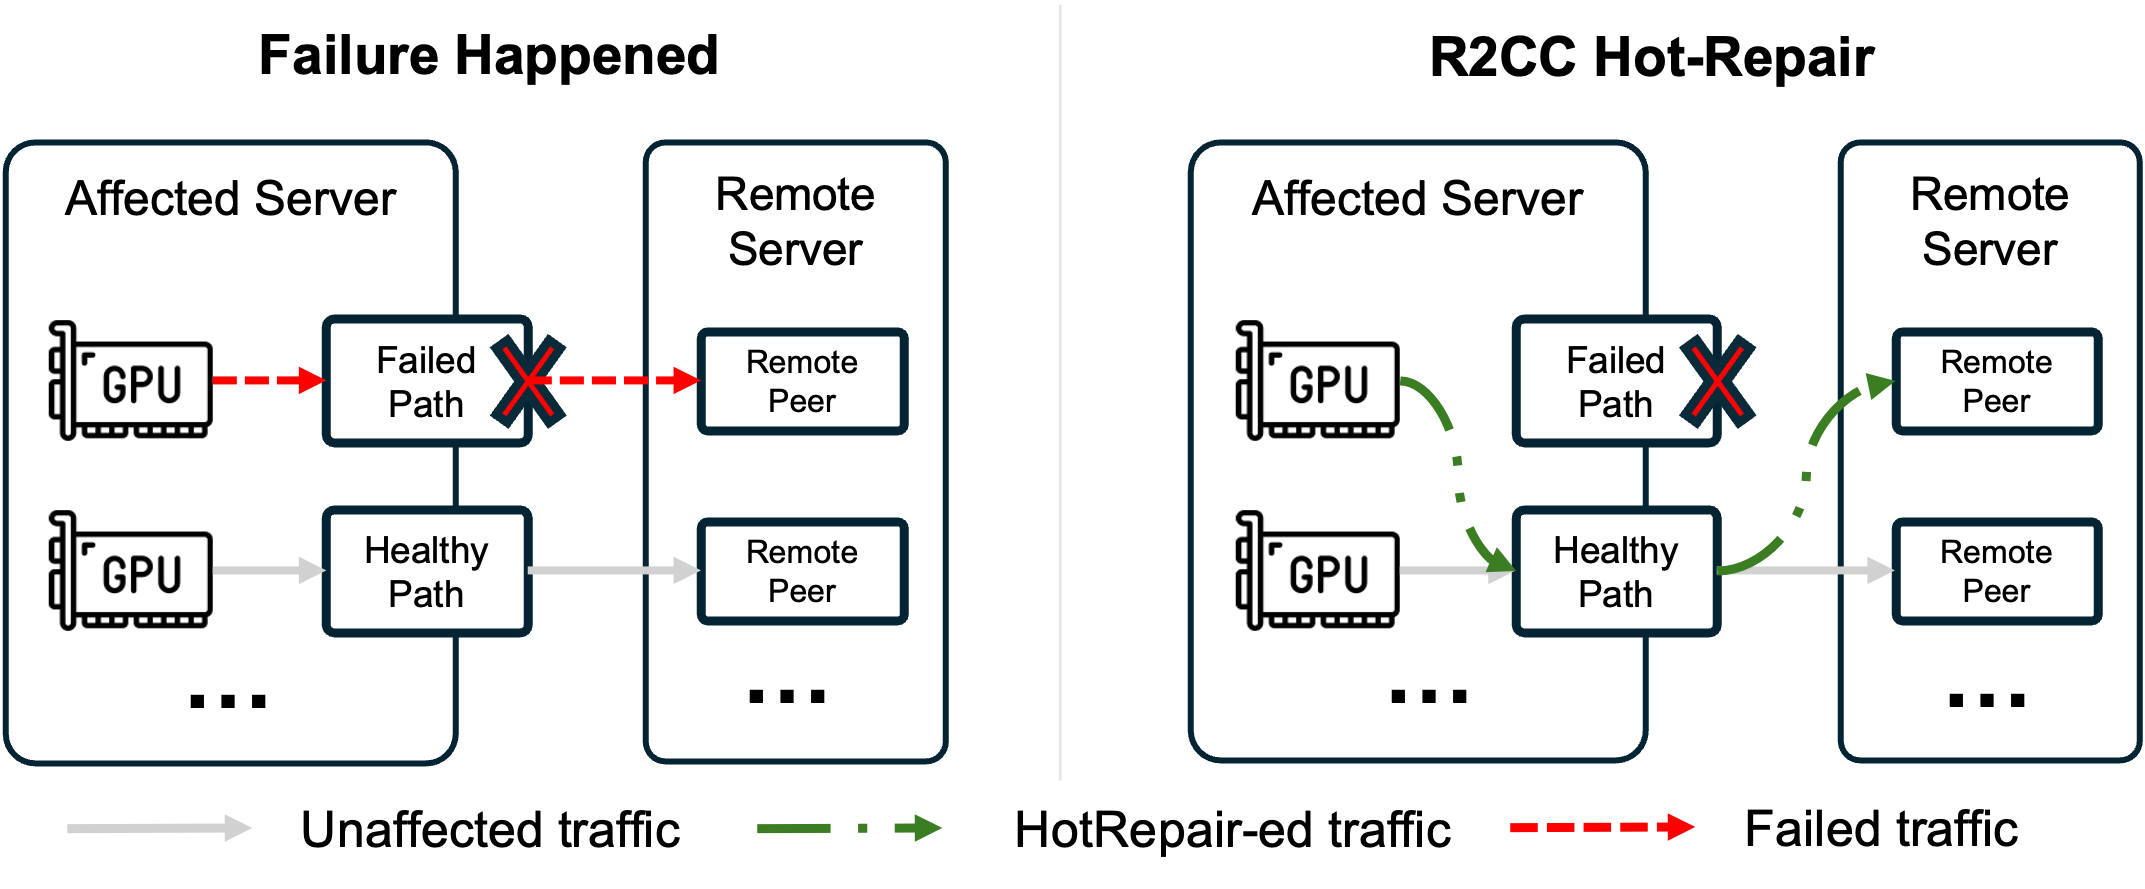
\includegraphics[width=1\linewidth]{figs/new-hotrepair.png}
    \vspace{-10pt}
    \tightcaption{\textbf{R2CC-HotRepair.} Affected traffic is switched to a pre-established healthy backup path after a failure.}
    \label{fig:new-hotrepair}
    \vspace{-2mm}
\end{figure}

\subsection{Degradation Signaling and Restore}
\label{sec:signal-restore}

As R2CC keeps NCCL's collective API unchanged, network degradation is exposed through a separate query, \texttt{r2ccCommGetDegradationState()}, scoped to the communicator. The framework can poll this query at its own control points and chosen frequency, typically between iterations or requests. Each call returns the degradation epoch, the current state, the affected path, and the residual bandwidth, allowing the upper layer to decide whether to reschedule, throttle, or escalate to a heavier-weight recovery.

Restore is off the hot path. After failover, the current collective continues on the backup path while R2CC periodically reprobes the affected path. Once the original path becomes usable again, R2CC revalidates or re-establishes the primary path and switches subsequent collectives back at collective boundaries, so the primary and backup connections never access the buffer concurrently. It then reverts the degraded topology adaptation and updates the degradation signal exposed to the framework.

\section{Failure-aware Schedule Optimization}
\label{sec:single-failure}

When a failure is hot repaired, all in-flight messages are migrated from the failed NIC to a backup connection, which must now share bandwidth with other GPUs. If the collective continues to use its original schedule, all traffic formerly on the failed NIC now flows into the backup NIC, effectively doubling its load and significantly slowing communication.

We show that such a performance bottleneck can be \textit{largely} mitigated via a failure-aware design for all collectives: (1) \textit{R2CC-Balance} is a simple but generic load-balancing technique on top of NCCL's existing schedules. It evenly distributes traffic across the remaining healthy NICs and works for all collectives. (2) \textit{R2CC-AllReduce} is a novel AllReduce schedule that further improves throughput under failures.

\begin{figure}
    \centering
    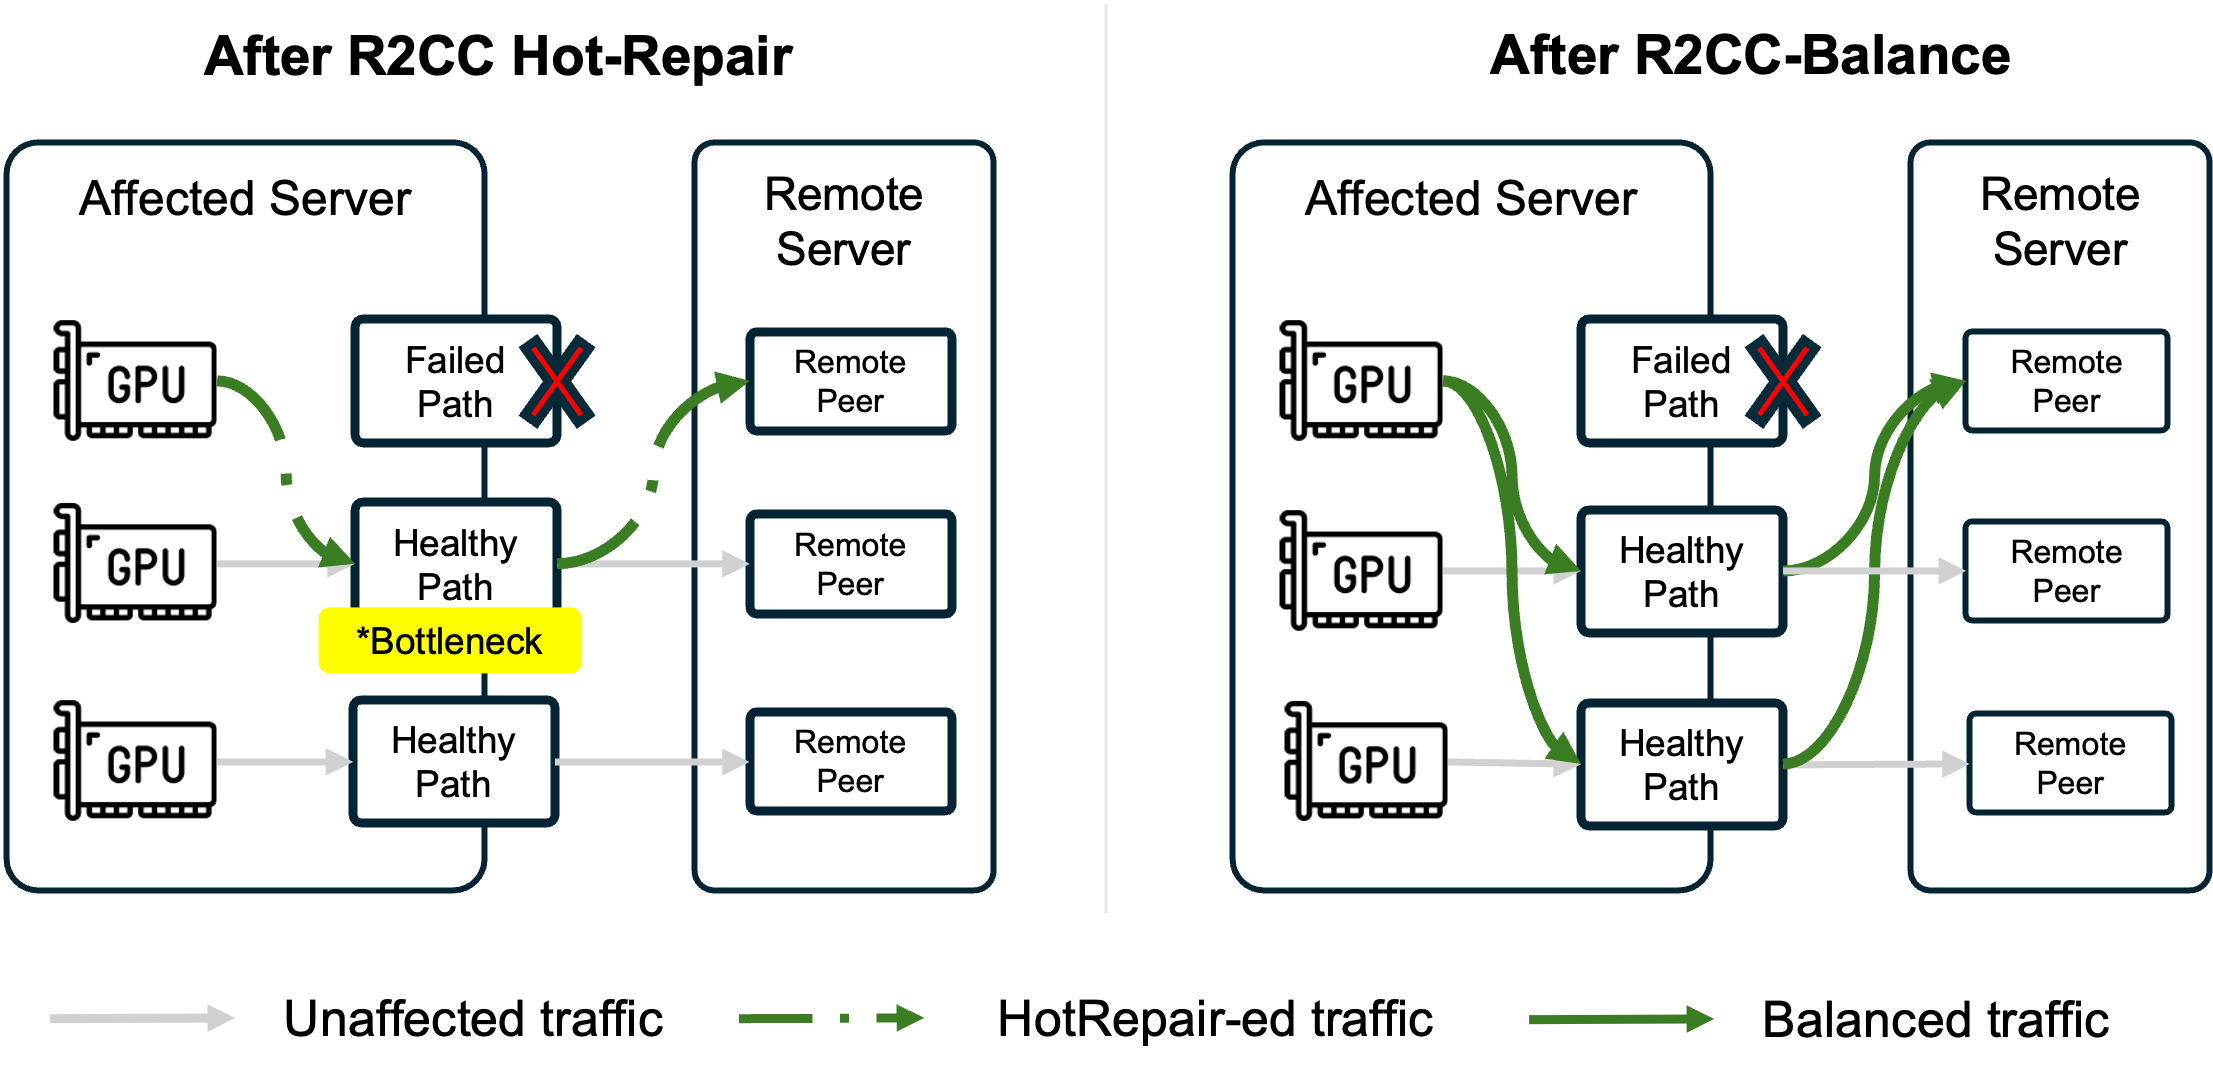
\includegraphics[width=0.97\linewidth]{figs/new-balance.png}
    \tightcaption{\textbf{R2CC-Balance.} After HotRepair, R2CC redistributes the repaired traffic across the remaining healthy paths to avoid overloading a single path.}
    \label{fig:new-balance}
    \vspace{-3mm}
\end{figure}

\subsection{R2CC Load Balancing}

\paragraph{R2CC-Balance.} As shown in Figure~\ref{fig:new-balance}, our first technique is a NIC-level load-balancing strategy that leaves NCCL collective algorithms unchanged. R2CC-Balance treats NCCL schedules as fixed and intervenes only at the network layer, making it applicable to all collective types. For each collective invocation, NCCL's algorithm (ring, tree, or hierarchical variants using NVSwitch multicast) determines the participating GPUs and the amount of inter-server data each server $i$ must send, denoted $D_i$. Rather than redesigning the collective, R2CC-Balance exploits one remaining degree of freedom: when a NIC or link on server $i$ fails, it redistributes the portion of $D_i$ that would have used the failed NIC across the healthy NICs in proportion to their available bandwidth.

\paragraph{PXN- and NUMA-aware load balancing.}
When rerouting traffic from a GPU to a backup NIC, R2CC can either send it directly over PCIe or relay it via NVLink using GPU proxy forwarding (PXN). R2CC selects between these options on a per-flow basis using a topology-aware policy. A failed NIC frees its PCIe lane from the affinity GPU, creating additional headroom that R2CC can exploit for detoured flows. Thus, R2CC prioritizes {\bf direct PCIe forwarding}: if the backup NIC is on the same NUMA node and its PCIe path has sufficient bandwidth headroom, the source GPU forwards traffic via PCIe. If the target NIC lies on a different NUMA node, R2CC compares the cost of traversing the CPU interconnect (e.g., QPI/UPI) with the NVLink headroom available for PXN. It then chooses the lower-cost path: either PCIe plus CPU-interconnect forwarding, or {\bf PXN forwarding} to a proxy GPU co-located with the target NIC.

\paragraph{Overhead Analysis.} NCCL's existing schedules already drive each server's cross-server traffic close to the semantic minimum for core collectives. For total data size $D_{\text{total}}$: a ReduceScatter retains only a $1/n$ shard and must send $\frac{n-1}{n}D_{\text{total}}$; an AllGather must receive the same amount; and in a Broadcast, the root sends $D_{\text{total}}$ while all others receive it. NCCL's ring algorithm realizes these lower bounds in homogeneous systems.

After a NIC failure, these volumes do not change: server $i$ must still exchange $D_i$ bytes, even though its aggregate NIC bandwidth is reduced to $B_i^{\text{rem}}$. Because these collectives inherently require $\Theta(D_{\text{total}})$ cross-server traffic, no schedule can substantially reduce $D_i$; the only leverage is how efficiently the remaining bandwidth is used. R2CC-Balance therefore redistributes the portion of $D_i$ originally routed through the failed NIC across the healthy NICs, allowing their combined throughput to approach $B_i^{\text{rem}}$. So completion time is dictated primarily by the reduced capacity of the slowest server.

\subsection{R2CC AllReduce}

Ring-based AllReduce is typically realized as a two-stage protocol (e.g., in NCCL and RCCL): A ReduceScatter over all GPUs followed by an AllGather over all GPUs, while tree-based AllReduce corresponds to a Reduction on a tree followed by a Broadcast on the same tree.

\begin{figure}[t]
   \centering
   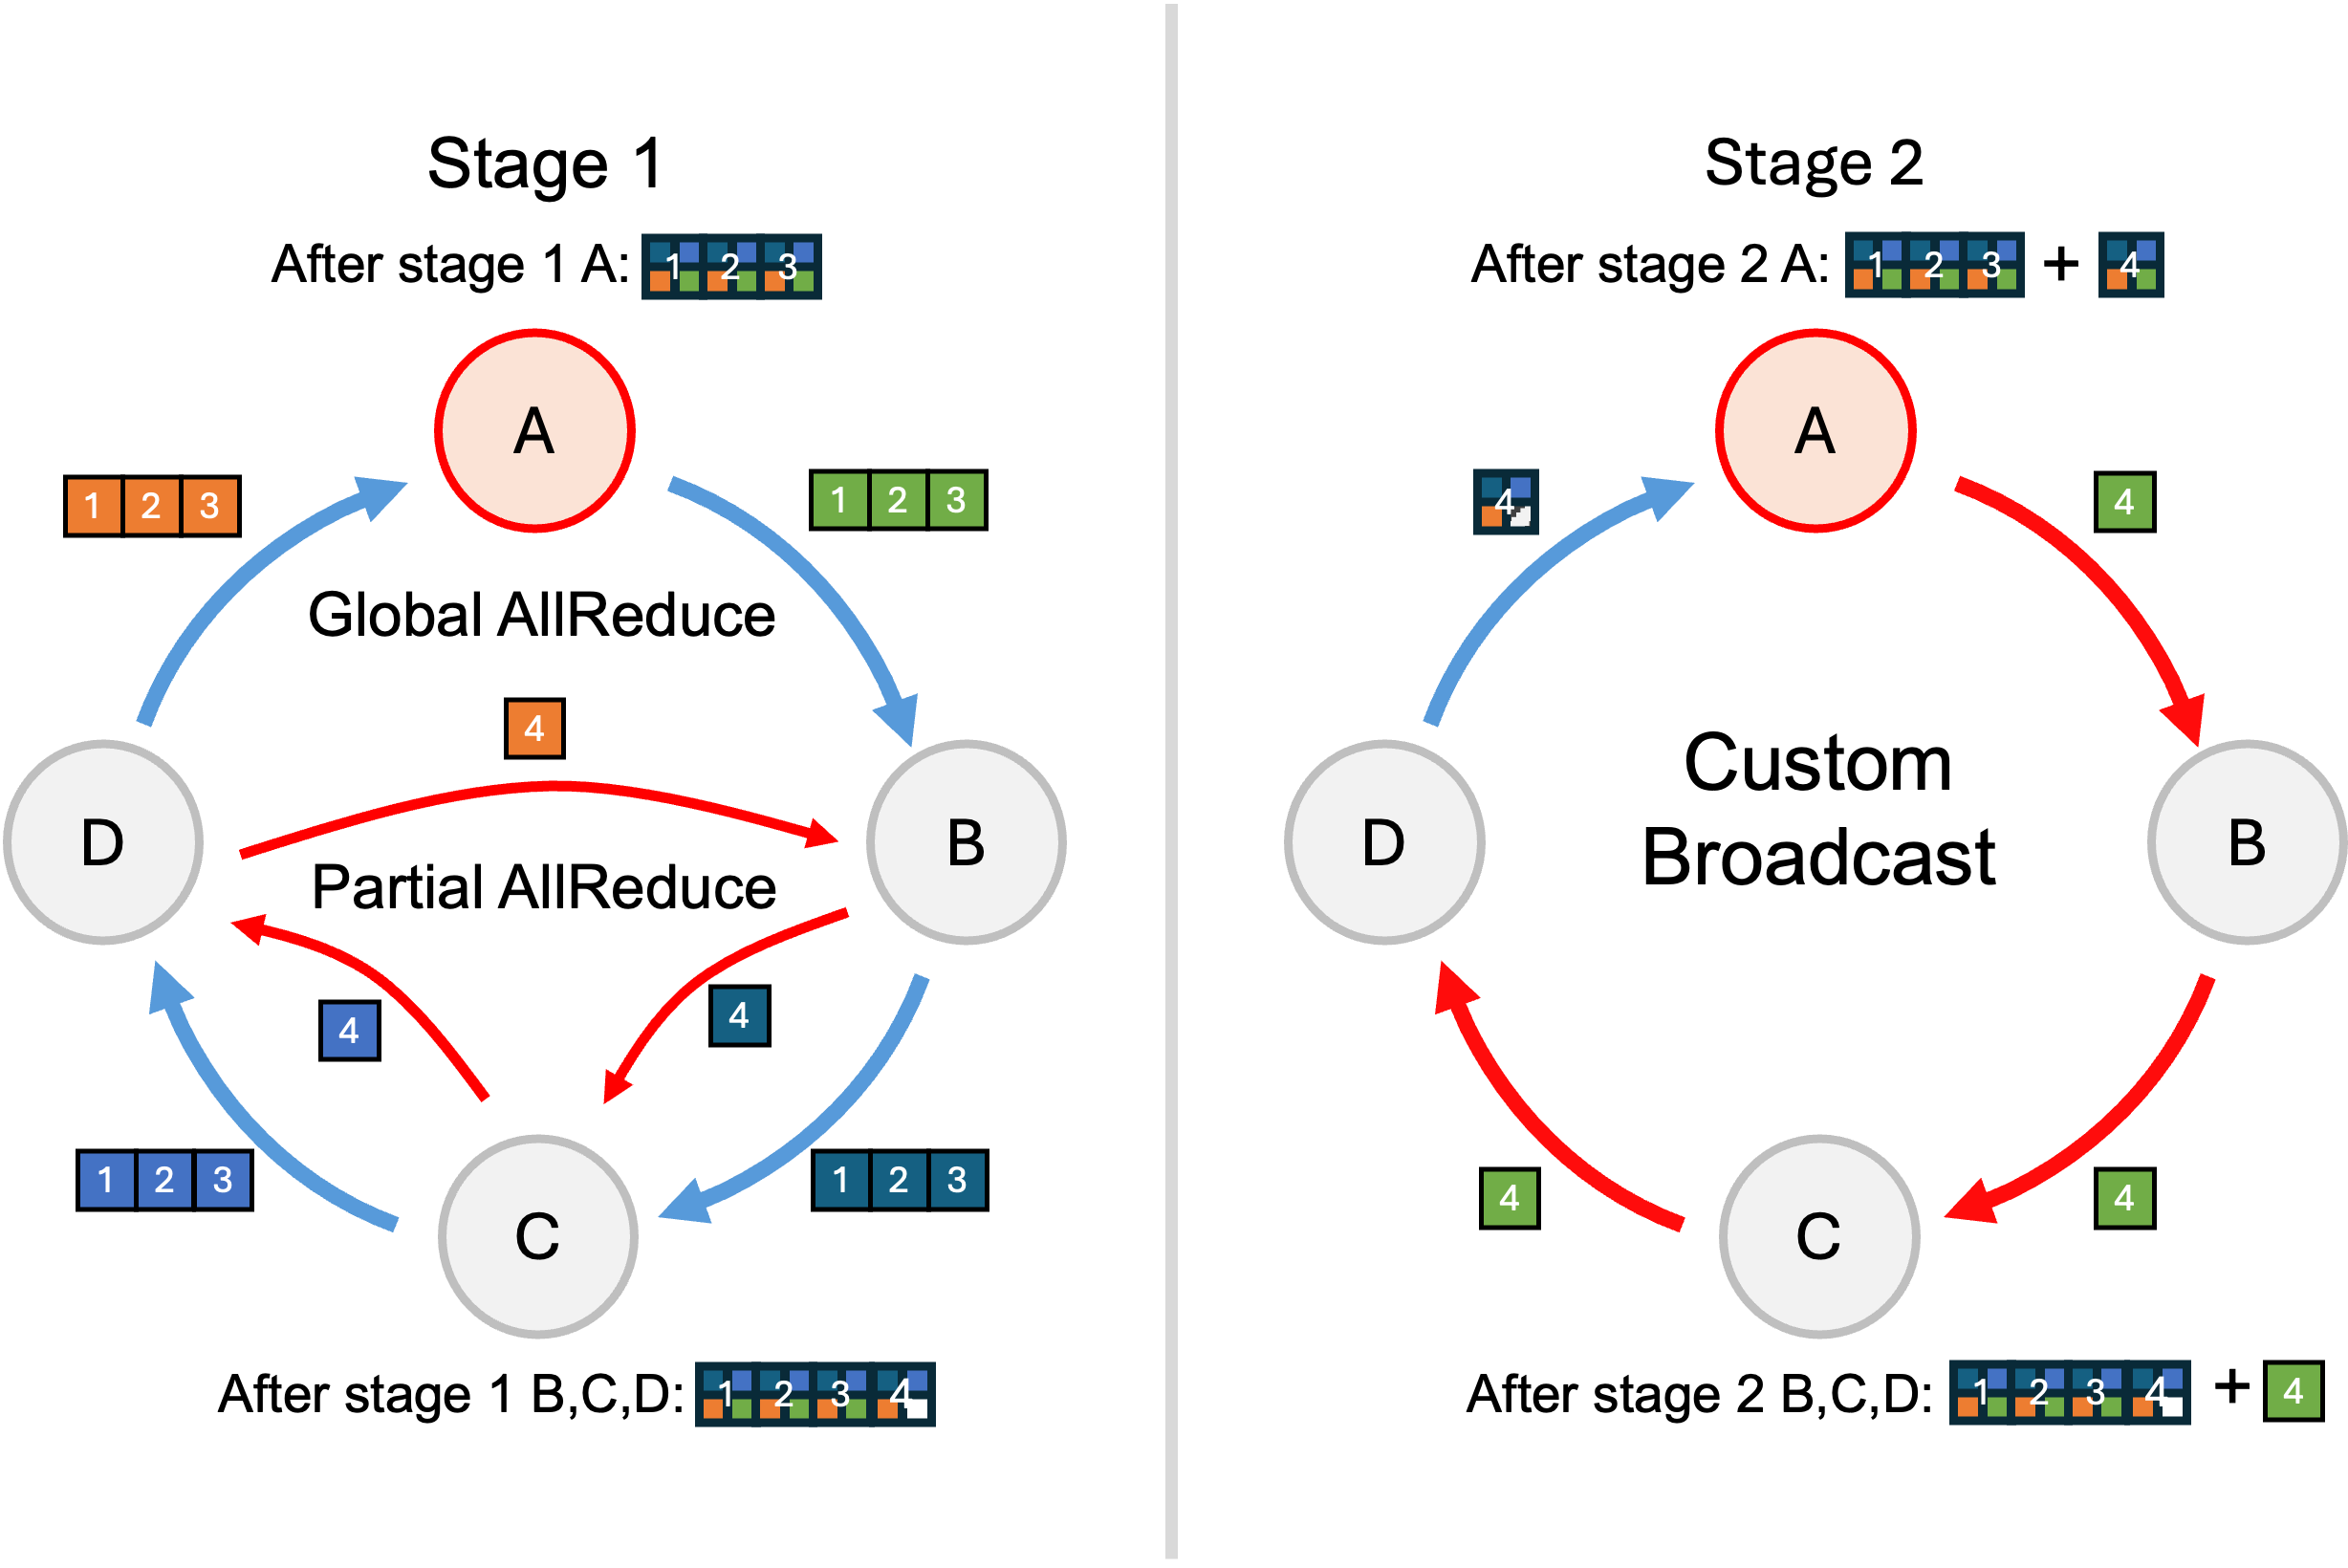
\includegraphics[width=1\linewidth]{figs/new-allreduce.png}
   \vspace{-15pt}
    \tightcaption{\textbf{R2CC-AllReduce reduces the degraded node’s load from $2D$ to $7/4D$.} In this 4-node example with lost-bandwidth fraction $1/4$, Stage~1 runs a global AllReduce with all 4 nodes on $3/4D$ and a partial AllReduce with 3 healthy nodes on $1/4D$, and Stage~2 broadcasts the $1/4D$ partial result back. Thus node $A$ carries $2\!\cdot\!3/4D + 1/4D = 7/4D$. Since the data and bandwidth in Stage 1 are proportional, the total completion times are nearly the same for each rank. }
    \label{fig:algorithm}
\end{figure}

To AllReduce $D$ size data per GPU, in ReduceScatter operation, a server must transmit all $D$ size data via its NIC, excluding the portion reduced onto itself; conversely, in AllGather, it must receive at least $D$ size data from the others. Because the two operations execute sequentially rather than concurrently, the peak load on a server consists of transmitting roughly $D$ during ReduceScatter and receiving roughly $D$ during AllGather, leading to a combined data volume of approximately $2D$.

In contrast, for an AllReduce operation, a key insight is that {\bf a server can wait for other nodes to complete a \textit{partial AllReduce} that excludes itself, and subsequently send and receive only the data it requires (broadcast) to satisfy the full operation demand}. Moreover, partial AllReduce can proportionally reduce the load on a specific server such as a server with a failed NIC, to improve the overall AllReduce performance. In practice, the failure server node retains some healthy NICs; we can allow it to participate in the global AllReduce across all ranks over a
subset of the data, while the remaining data are handled by a
partial AllReduce that excludes the failure node.

\paragraph{R2CC-AllReduce.} Based on the above insights, we propose a novel AllReduce algorithm (Figure~\ref{fig:algorithm}). When NIC failures induce inter-node bandwidth heterogeneity, we partition the AllReduce into two stages:

(1) \textit{The first stage} executes a global AllReduce and a partial AllReduce concurrently. The global AllReduce spans all servers, including the one with the failed NIC, and is therefore throttled by the reduced effective bandwidth of the affected server. In parallel, the partial AllReduce excludes the failure node and utilizes the remaining capacity of the healthy servers to process its share of data at full speed.

(2) \textit{The second stage} executes a tailored broadcast that completes the partial-AllReduce plus broadcast path. This process comprises a broadcast initiated from the failure server node, a pipelined ring broadcast across the healthy servers, and the final delivery of the partial-AllReduce result from the last node in the ring back to the failure node, ensuring that all servers obtain the full correct AllReduce result.

\smallskip\noindent\textbf{Data partition and implementation.} Let $D$ be the per-node AllReduce data size, $B$ the per-node bandwidth, $n \geq 2$ the number of nodes, $X \in (0, 1)$ the fraction of bandwidth lost on the failed node, and $Y \in [0, 1]$ the fraction of data routed through the partial AllReduce. In Stage~1, a global AllReduce over all $n$ nodes on $(1-Y)D$ bottlenecked by the failed node's $(1-X)B$ runs concurrently with a partial AllReduce over the $n-1$ healthy nodes on $YD$ using their reserved $XB$; Stage~2 broadcasts the $YD$ partition back to the failed node over its $(1-X)B$:
\begin{align*}
T_1(Y) &= \frac{2(n-1)}{n} \cdot \frac{(1-Y)D}{(1-X)B}, \\
T_2(Y) &= \frac{2(n-2)}{n-1} \cdot \frac{YD}{XB}, \\
T_3(Y) &= \frac{YD}{(1-X)B}.
\end{align*}
The total completion time $T(Y) = \max(T_1(Y), T_2(Y)) + T_3(Y)$ is minimized at
$$Y^* = \frac{(n-1)^2 X}{n^2 - 2n + X}.$$
Because $Y^*$ produces awkward byte offsets that complicate buffer management and memory alignment, we instead adopt the simpler rule $Y = X$, whose approximation gap satisfies
$$\frac{T(X) - T(Y^*)}{T(Y^*)} < Y^* - X \leq \frac{1}{4n(n-2)},$$
which decays as $O(1/n^2)$ and reaches at most $1.2\%$ at $n = 4$. The full derivation and per-$(n, X)$ values are given in Appendix~\ref{appendix:allreduce-math}. R2CC-AllReduce therefore adopts $Y = X$, and we use $T(X)$ to denote its completion time hereafter.

\textbf{Comparison with no-failure time.} To quantify the failure-induced overhead of each variant, we compare against the no-failure ring AllReduce time $T_{\text{nf}} = \frac{2(n-1)D}{nB}$. Direct computation gives
$$\frac{T_{\text{Balance}} - T_{\text{nf}}}{T_{\text{nf}}} = \frac{X}{1-X}, \qquad \frac{T(X) - T_{\text{nf}}}{T_{\text{nf}}} = \frac{nX}{2(n-1)(1-X)}.$$
The ratio of Balance's overhead to R2CC-AllReduce's overhead is exactly $\frac{2(n-1)}{n}$, the ring AllReduce efficiency factor, which approaches $2$ as $n \to \infty$. Thus R2CC-AllReduce asymptotically halves the failure-induced overhead relative to R2CC-Balance. Figure~\ref{fig:overhead-compare} plots both overheads across the full range of $X$: at $X = 50\%$ and $n = 16$, R2CC-Balance incurs a 100\% overhead while R2CC-AllReduce with $Y = X$ cuts it to 53.3\%.

\begin{figure}[t]
    \centering
    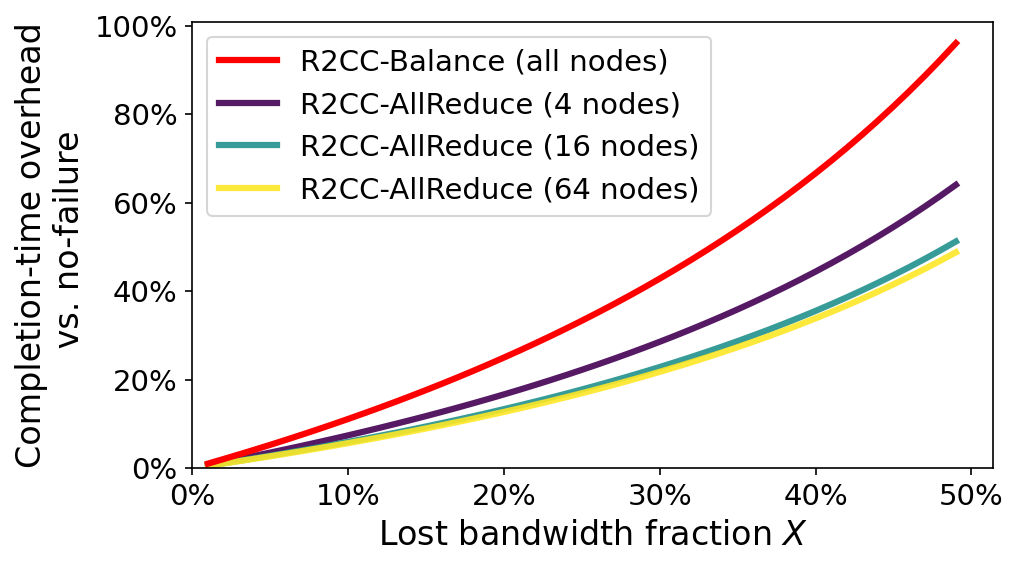
\includegraphics[width=0.85\columnwidth]{figs/overhead.png}
    \vspace{-5pt}
    \tightcaption{\textbf{Overhead Analysis.} Completion-time overhead vs.\ no-failure as a function of lost bandwidth fraction $X$.}
    \label{fig:overhead-compare}
    \vspace{-2mm}
\end{figure}

\paragraph{Optimize Scheduling Under Multi-Failure.} Beyond the single-failure scenario, handling multi-failure case is discussed in Appendix~\ref{sec:multi-failure}.
